\section{Introducción}  %RESUMEEEEN
\noindent En esta practica realizaremos diversas mezclas para determinar su carácter (exotérmico o endotérmico), así como determinaremos el equivalente en agua del calorímetro usando para ello agua destilada tanto fría como caliente. Y por último, determinaremos la entalpía de neutralización tanto de un ácido fuerte con una base fuerte como un ácido débil con una base fuerte.

\section{Inventario}
Para esta práctica hemos usado:

\begin{multicols}{2}
    \begin{itemize}
        \item Un calorímetro
        \item Una pipetas graduadas
        \item Una propipeta
        \item Un termómetro
        \item 4 tubos de ensayo
        \item 2 vasos de precipitados
        \item 2 pipetas pasteur
        \item Una varilla
        \item 2 espátulas
        \item 2 probetas
        \item Un recipiente negro para pesar diversos sólidos en la balanza
        \item Sólidos: azúcar, \ce{CaO}, \ce{NaCl}, \ce{KNO_3}
        \item Líquidos: \ce{HCl}, \ce{H_2SO_4}, \ce{HNO_3}, \ce{NaOH}, \ce{CH_3COOH}
    \end{itemize}
\end{multicols}

\vspace{0.8cm}

Podemos ver parte de lo nombrado anteriormente en las siguientes fotografías:

\begin{figure}[H]
    \centering
    \hspace*{-2.3cm}
        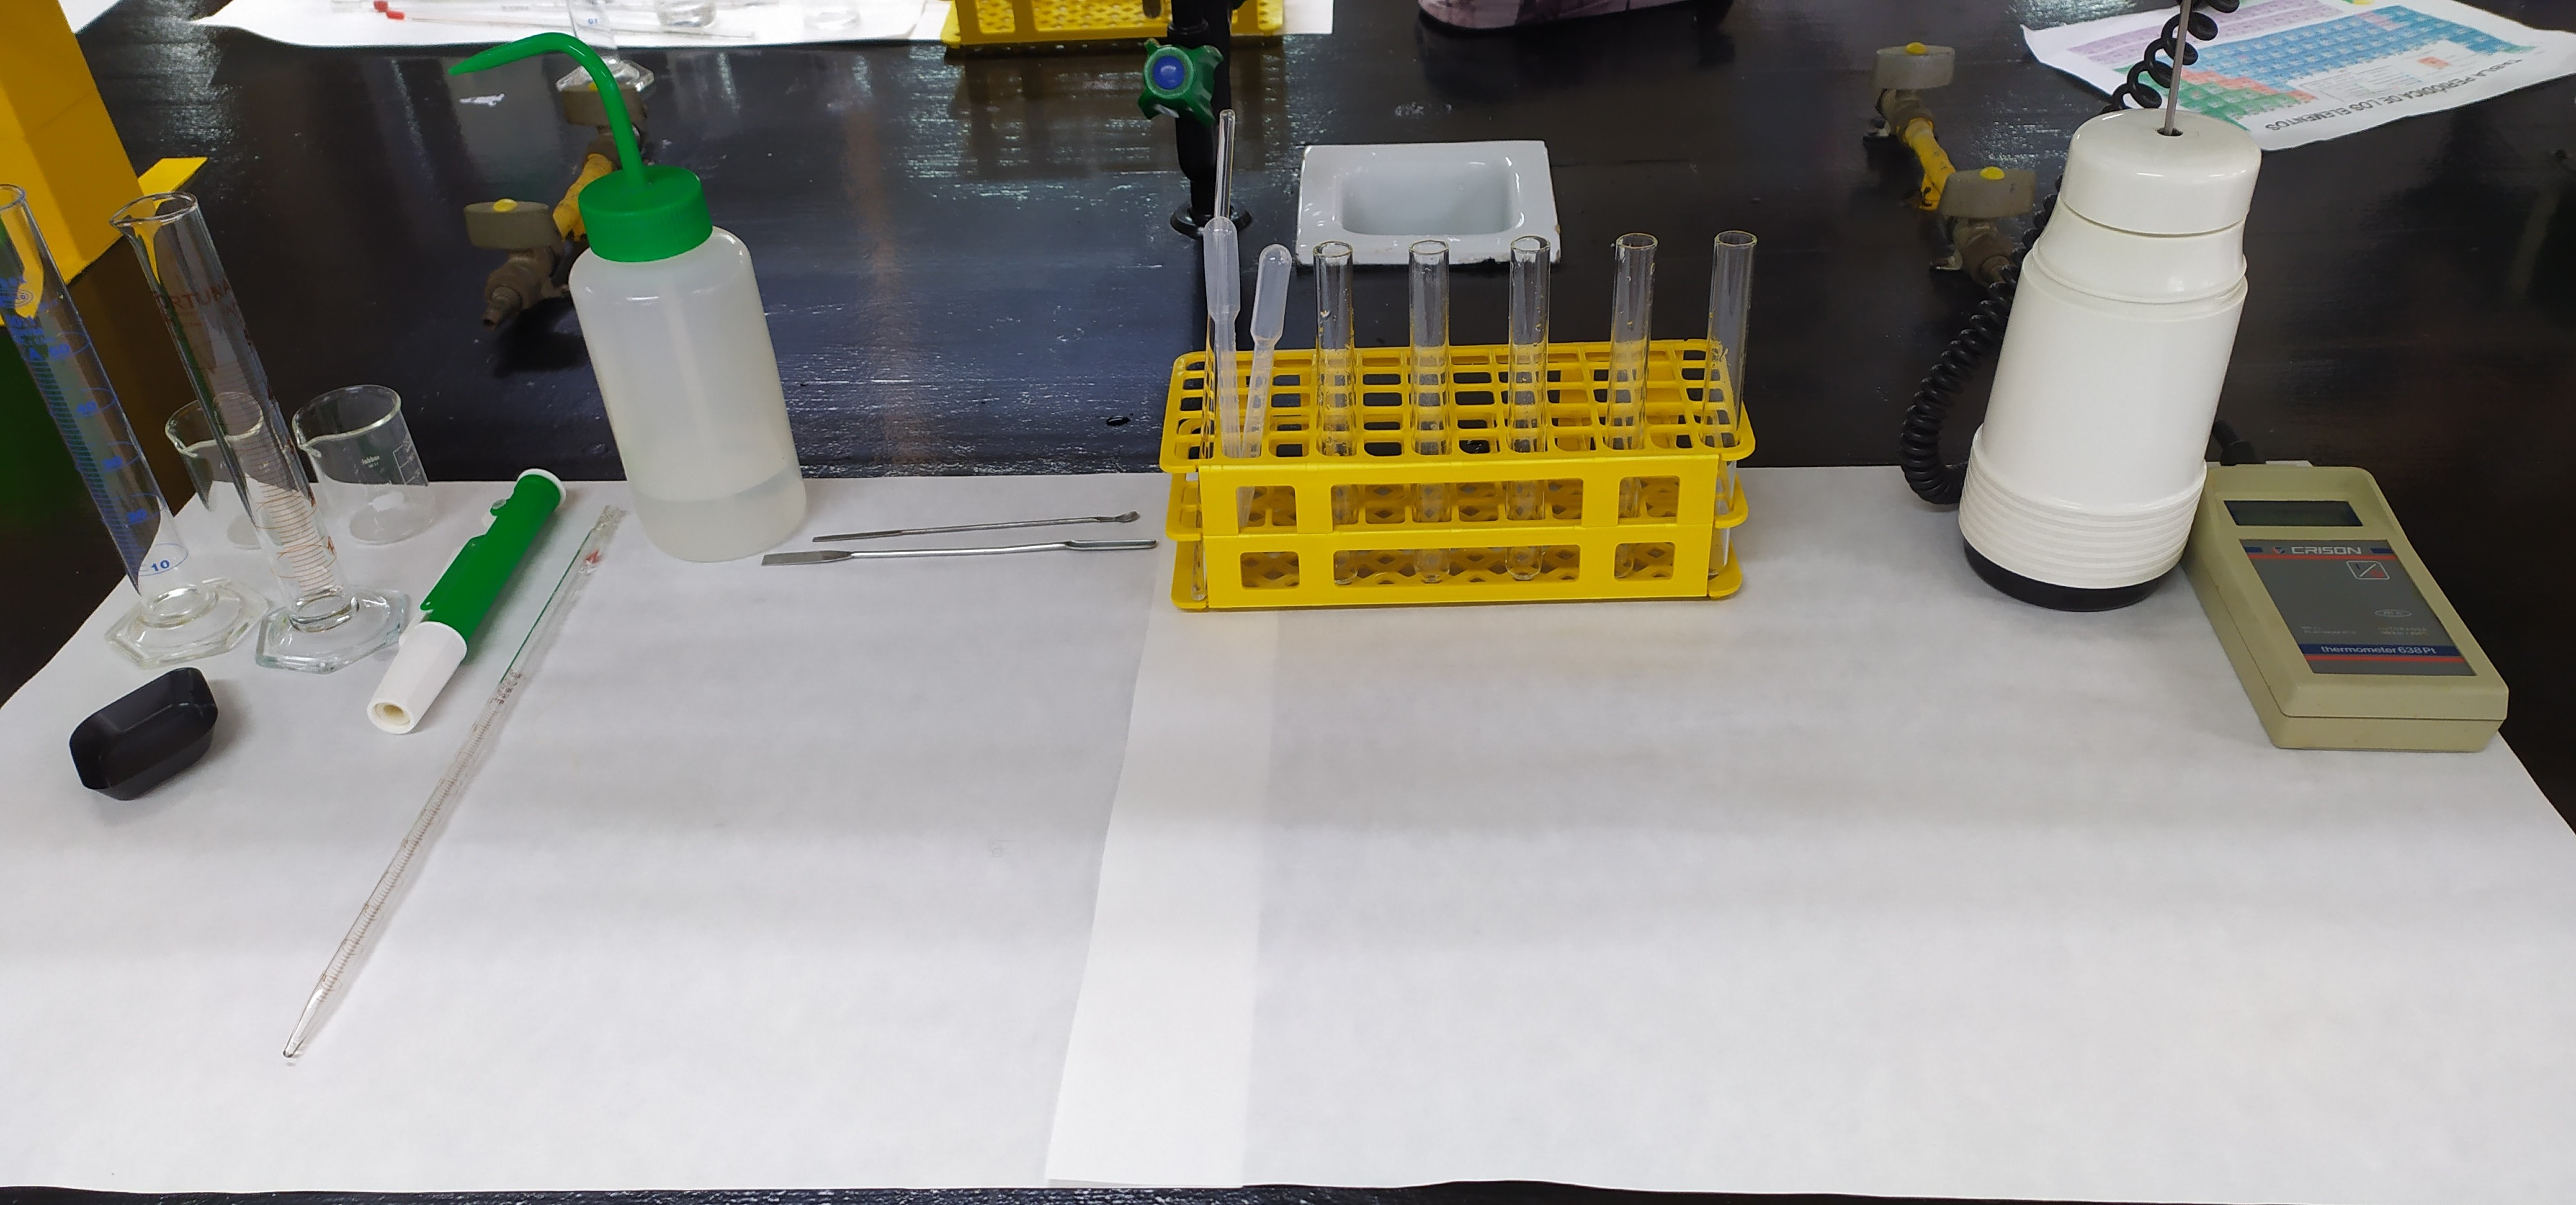
\includegraphics[scale = 0.06]{fotos/mesa2.jpg}
        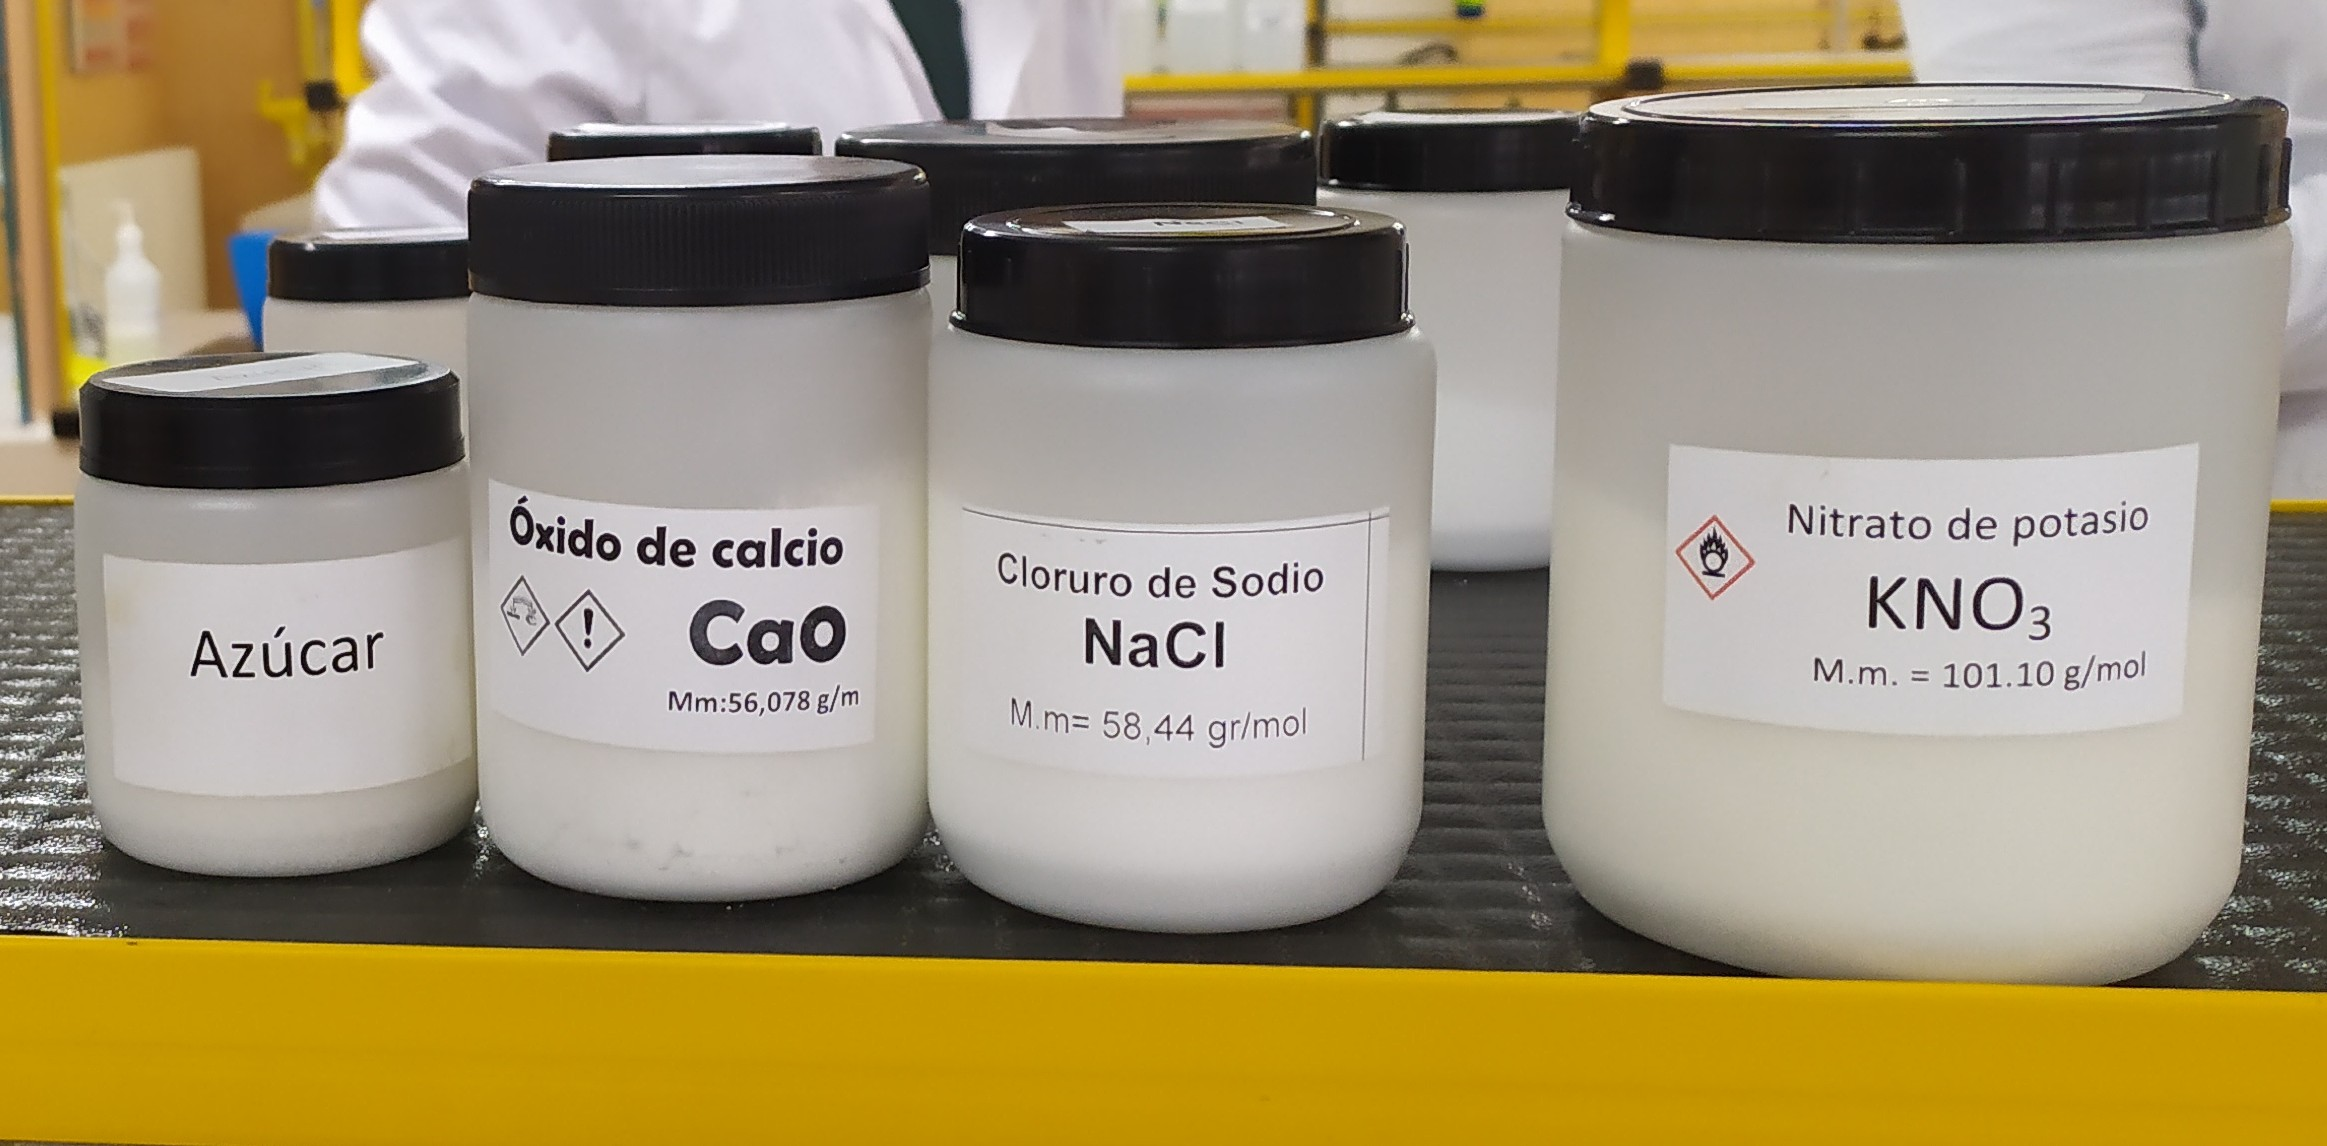
\includegraphics[scale = 0.08]{fotos/soli2.jpg}
    \hspace*{-2.3cm}
    \caption{A la izquierda el material usado y a la derecha los sólidos empleados}
\end{figure}

\clearpage

\section{Procedimiento} 
\noindent En la \textcolor{red}{primera parte} hemos realizado una serie de mezclas de compuestos en tubos de ensayo para determinar los distintos cambios de temperatura. A continuación expongo las distintas mezclas:

\vspace{0.3cm}

i) Mezcla de 0,5 g de óxido de calcio con 3 mL de agua: \newline
\textbf{Proceso exotérmico ($\Delta{T} > 0$)}

\vspace{0.2cm}

ii) Mezcla de un poco de azúcar con unas gotas de ácido sulfúrico concentrado:\newline \textbf{Proceso exotérmico ($\Delta{T} > 0$)}

\vspace{0.2cm}

iii) Mezcla de 0,5 g de nitrato de potasio sólido y 3 mL de agua: \newline
\textbf{Proceso endotérmico ($\Delta{T} < 0$)}

\vspace{0.2cm}

iv) Mezcla de 3 mL
de agua y ácido nítrico concentrado: \newline
\textbf{Proceso exotérmico ($\Delta{T} > 0$)}

\vspace{0.2cm}

v) Mezcla de 0,5 g de cloruro
de sodio y 3 mL de agua: \newline
\textbf{Proceso exotérmico ($\Delta{T} > 0$)}

\vspace{0.3cm}
\noindent Esta parte nos ha servido para tener una primera toma de contacto con lo que vamos a realizar a lo largo de esta práctica. \\

\vspace{0.3cm}

\noindent Ahora vamos a centrarnos en la \textcolor{red}{segunda parte}, en la determinación del equivalente en agua del calorímetro. \\

\noindent En primer lugar, hay que climatizar el calorímetro con agua fría para poder obtener unos resultados próximos a la realidad. Y todos los procesos descritos a continuación tendremos que repetirlos 3 veces para que el resultado sea más preciso. \\

\noindent Tendremos que colocar 50 mL de agua muy fría en el calorímetro agitándolo hasta alcanzar el equilibrio, que en nuestro caso se alcanza a 7.8$^o$C ($T_1$). Una vez alcanzado el equilibrio añadimos 50 mL de agua destilada a temperatura ambiente, previamente medido en una probeta (con una temperatura de 17.5$^o$C, $T_2$), y alcanzamos una temperatura de 12$^o$C ($T_f$) una vez estabilizada la mezcla. 

\clearpage

\noindent Una vez con estos datos podemos determinar el equivalente en agua del calorímetro(W) usando las siguientes fórmulas:

\vspace{0.3cm}

\begin{equation} \label{cedido}
    q_{cedido~ agua~ caliente} = m_{agua~ caliente}\cdot{c_e}\cdot{(T_f - T_2)}
\end{equation}

\begin{equation} \label{ganado}
    q_{\text{ganado~ agua~ fría}} = m_{\text{agua~ fría}}\cdot{c_e}\cdot{(T_f - T_1)}
\end{equation}

\begin{equation} \label{cal}
    q_{\text{calorímetro}} = W\cdot{c_e}\cdot{(T_f - T_1)}
\end{equation}

\begin{equation} \label{sumat}
    q_{cedido~ agua~ caliente} + q_{\text{ganado~ agua~ fría}} + q_{\text{calorímetro}} = 0
\end{equation}

\vspace{0.4cm}

\noindent Para obtener el valor de W sustituimos en la ecuación \eqref{sumat} el valor de las q's definidas en las ecuaciones \eqref{cedido}, \eqref{ganado} y \eqref{cal}. Obtenemos así esta ecuación, de la que podemos cancelas las $c_e$:

\[ m_{agua~ caliente}\cdot{c_e}\cdot{(T_f - T_2)} + m_{\text{agua~ fría}}\cdot{c_e}\cdot{(T_f - T_1)} + W\cdot{c_e}\cdot{(T_f - T_1)} = 0\]

\noindent Despejamos la W y se nos queda esta ecuación:

\[ W = \frac{-m_{agua~ caliente}\cdot{(T_f - T_2)} - m_{\text{agua~ fría}}\cdot{(T_f - T_1)}}{T_f - T_1)}\]

\vspace{1cm}

\begin{table}[h]
    \centering
\begin{tabular}{ | c | c | c | c |} 
    \hline
    \multicolumn{4}{ |c| }{Resultados} \\
    \hline
    $T_1$ $(^oC)$ & 7.8 & 5.5 & 4.2 \\  
    $T_2$ $(^oC)$ & 15 & 17.5 & 17.5  \\
    $T_f$ $(^oC)$ & 12 & 11.1 & 10.1 \\
    \hline
    W (J)  & 15.48 & 7.14 & 12.71 \\  

    \hline
\end{tabular}
    \caption{Tabla de los datos obtenidos  tras las mediciones y cálculos}
    \label{tabla-temp y w}
\end{table}

\vspace{0.4cm}

\noindent A continuación abordaremos el \textcolor{red}{tercer punto} de esta práctica, que es la determinación de la entalpía de neutralizar un ácido fuerte con una base fuerte.\\


\noindent Para hacer esto, medimos en una probeta 50 mL de  disolución 2 M de hidróxido de sodio (NaOH) y lo colocamos en el calorímetro. A continuación, introducimos otros 50 mL de ácido clorhídrico 2M (HCl). Ambas disoluciones por separado están a temperatura ambiente (unos 16$^o$C) y tras reaccionar en el calorímetro obtenemos una temperatura resultante de 28.7$^o$C.\\


\noindent Una vez que sabemos la temperatura de reacción, la entalpía de reacción la podemos sacar de la fórmula \eqref{entalps}, teniendo los valores siguientes: $c_e$ = 4.18, $m_{mezcla}$ = 100 g, W = 11.78 J (la media de todos los trabajos obtenidos previamente) y $\Delta{T}$ = 28.7 - 16 = 12.7$^o$C (temperatura de reacción menos la ambiente en la primera medida). Por lo tanto, de la ecuación \eqref{entalps} podemos despejar la entalpía de reacción ($\Delta{H_{reaccion}}$ fácilmente y se pueden sustituir los valores par obtener dicho valor. Pero puesto que en esta parte realizamos también 3 medidas para obtener una mayor precisión, voy a hacer una tabla para que se vean mejor los datos y los resultados obtenidos.

\vspace{0.4cm}

\begin{equation} \label{entalps}
    \Delta{H_{reaccion}} + m_{mezcla}\cdot{c_e}\cdot{\Delta{T}} + W\cdot{c_e}\cdot{\Delta{T}} = 0
\end{equation}

\vspace{0.4cm}

\begin{table}[H]
    \centering
\begin{tabular}{ | c | c | c | c |} 
    \hline
    \multicolumn{4}{ |c| }{Resultados} \\
    \hline
    $T_r$ $(^oC)$ & 28.7 & 30.3 & 29.8 \\  
    $\Delta{T}$ $(^oC)$ & 12.7 & 14.3 & 13.8  \\
    \hline
    $\Delta{H_r}$ $(J)$ & -5933.95 & -6681.54 & -6447.92 \\   

    \hline
\end{tabular}
    \caption{Tabla de las entalpías obtenidas}
    \label{entalp}
\end{table}


\noindent Finalmente, nos encontramos ya en la \textcolor{red}{última parte} de la práctica, que es bastante parecida al apartado anterior pero en el ácido fuerte lo cambiamos por un ácido débil. \\

\noindent Ahora, mediremos 50 mL de hidróxido sódico 2M y lo añadimos en el calorímetro, para a continuación repetir el mismo proceso con 50 mL de ácido acético 2M ($CH_3COOH$) . En esta parte usaremos también la ecuación \eqref{entalps}. Y haremos otra tabla para ver los datos de las 3 mediciones realizadas.

\begin{table}[H]
    \centering
\begin{tabular}{ | c | c | c | c |} 
    \hline
    \multicolumn{4}{ |c| }{Resultados} \\
    \hline
    $T_r$ $(^oC)$ & 28.3 & 28 & 28.1 \\  
    $\Delta{T}$ $(^oC)$ & 12.3 & 12 & 12.1  \\
    \hline
    $\Delta{H_r}$ $(J)$ & -5748.09 & -5607.89 & -5654.62 \\   

    \hline
\end{tabular}
    \caption{Tabla de las entalpías obtenidas}
    \label{entalp-2}
\end{table}

\clearpage

\section{Cuestiones}

\noindent\textcolor{BlueViolet}{\textbf{\textit{a) Escriba las reacciones correspondientes a los procesos estudiados en el primer apartado, indicando si son endotérmicos o exotérmicos.}}}\\


    \vspace{0.1cm}
    
     Este apartado ya lo he completado parcialmente en el procedimiento, lo único que falta es poner la correspondiente reacción:\\
    
    \vspace{0.2cm}
    
    i)$~ CaO(g) + H_2O(l) ~\rightleftharpoons ~Ca(OH)_2$
    
    \vspace{0.2cm}
    
    ii)$~ C_{12}H_{22}O_{11}(s) + H_2O(l) ~\rightleftharpoons ~ H_2O(g) + C(s)$
    
    \vspace{0.2cm}
    
    iii)$~ H_2O(l) + KNO_3(s) ~\rightleftharpoons ~ HNO_3 + KOH$
    
    \vspace{0.2cm}
    
    iv)$~ HNO_3(l) + H_2O(l) ~\rightleftharpoons ~ NO_3^- + H_3O^+$
    
    \vspace{0.2cm}
    
    v)$~ NaCl(s) + H_2O(l) ~\rightleftharpoons ~ NaOH + HCl$\\
    
    \vspace{0.3cm}

\noindent\textcolor{BlueViolet}{\textbf{\textit{b) Determine los valores de la entalpía de neutralización de las dos reacciones
estudiadas.}}}\\

    \vspace{0.2cm}
    
    Las entalpías obtenidas podemos observarlas en los cuadros \ref{entalp} y \ref{entalp-2}\\
    
    \vspace{0.4cm}

\noindent\textcolor{BlueViolet}{\textbf{\textit{c) Calcule teóricamente la entalpía de la reacción de neutralización y compare el
resultado teórico con los resultados experimentales obtenidos.}}}\\

 Calculemos la entalpía de reacción teóricamente para ver si nuestros datos experimentales son correctos:\\
\[\Delta{H_{r}} = \Delta{H_{f}(H_2O)} - \Delta{H_{f}(H^+)} - \Delta{H_{f}(OH^-)} = -285.8 - 0 - (-230) = -55 kJ\]

 Podemos observar que los valores experimentales obtenidos a lo largo de la práctica se aproximan bastante al teórico calculado.













